%=========================================================
% Slide-wise Handout : Technical Terms
% Modern Computing and Python Programming (26ESCC106)
% Module 1 : Evolution of Computing (Text Book 1: 1.1 - 1.1.2)
% Compile using XeLaTeX:  latexmk -xelatex handout.tex
%=========================================================

\documentclass[11pt,a4paper]{article}

%---------------------------------------------------------
% Packages
%---------------------------------------------------------
\usepackage[margin=2cm,headheight=28pt,headsep=12pt]{geometry}
\usepackage{fontspec}
\setmainfont{Times New Roman}
\usepackage{amsmath,amssymb}
\usepackage{graphicx}
\usepackage{booktabs}
\usepackage{array}
\usepackage{tabularx}
\usepackage{enumitem}
\usepackage{fancyhdr}
\usepackage{xcolor}
\usepackage[most]{tcolorbox}
\usepackage{tikz}
\usetikzlibrary{arrows.meta,positioning,shapes.geometric,shapes.misc,shapes.symbols,fit,calc,backgrounds,decorations.pathreplacing}
\usepackage[hidelinks]{hyperref}
\usepackage{titlesec}

\setlist{nosep,leftmargin=*}
\setlength{\parindent}{0pt}
\setlength{\parskip}{4pt}

%---------------------------------------------------------
% Header / Footer
%---------------------------------------------------------
\pagestyle{fancy}
\fancyhf{}
\fancyhead[L]{
\includegraphics[height=22pt]{images/MITE_logo.png}}
\fancyhead[C]{\small\textbf{Modern Computing and Python Programming (26ESCC106)}\\ \footnotesize Module 1 Handout: Technical Terms, Slide by Slide}
\fancyhead[R]{\small Manjunath Prasad H. R.}
\fancyfoot[C]{\small Page \thepage}
\renewcommand{\headrulewidth}{0.6pt}

%---------------------------------------------------------
% Slide heading and term box
%---------------------------------------------------------
\titleformat{\section}{\large\bfseries}{}{0pt}{}
\titlespacing*{\section}{0pt}{10pt}{4pt}

\newcommand{\slide}[2]{%
  \section*{\colorbox{black}{\textcolor{white}{\,Slide #1\,}}\; #2}%
  \addcontentsline{toc}{subsection}{Slide #1: #2}}

\newtcolorbox{termbox}[1]{enhanced,breakable,colback=white,colframe=black,
  colbacktitle=black!10,coltitle=black,fonttitle=\bfseries,
  boxrule=0.5pt,arc=1pt,left=5pt,right=5pt,top=3pt,bottom=3pt,
  title={#1},before skip=5pt,after skip=5pt}

% \term{Name}{Definition}{Description}
\newcommand{\term}[3]{%
\begin{termbox}{#1}
\textbf{Definition:} #2\par
\ifx&#3&\else\textbf{Description:} #3\fi
\end{termbox}}

\newcommand{\noterms}[1]{\textit{#1}\par}

\tikzset{
  box/.style={draw,rounded corners=2pt,align=center,font=\small,minimum height=0.8cm,inner sep=4pt},
  pc/.style={draw,minimum width=1.1cm,minimum height=0.7cm,font=\scriptsize,align=center},
  arr/.style={-{Stealth[length=2.5mm]},thick},
  darr/.style={{Stealth[length=2.5mm]}-{Stealth[length=2.5mm]},thick},
}

%=========================================================
\begin{document}
%=========================================================

\begin{center}
{\LARGE\bfseries Module 1: Evolution of Computing}\\[4pt]
{\large Slide-wise Handout of Technical Terms}\\[4pt]
Modern Computing and Python Programming (26ESCC106)\\
Text Book 1: Kai Hwang, Geoffrey C. Fox and Jack J. Dongarra, \textit{Distributed and Cloud Computing}, Morgan Kaufmann, 2012 (Sections 1.1, 1.1.1, 1.1.2)\\[6pt]
\textbf{Manjunath Prasad H. R.}, Assistant Professor, Department of AIML, MITE
\end{center}

\begin{tcolorbox}[colback=black!5,colframe=black,boxrule=0.5pt,arc=1pt]
\textbf{How to use this handout.} Each heading matches one slide of the lecture deck (the number in the black box is the slide number shown at the bottom-right of the slide). Under each heading, the technical terms that appear on that slide are defined and explained in simple language. Diagrams are given wherever a picture makes the idea easier to understand. Terms that are explained in detail later in the course are marked \textit{(covered later)}.
\end{tcolorbox}

\tableofcontents
\clearpage

%=========================================================
\part*{Part A: Course Overview Slides}
\addcontentsline{toc}{section}{Part A: Course Overview Slides (Slides 1--19)}
%=========================================================

\slide{1}{Title Slide}
\noterms{No technical terms on this slide.}

\slide{2}{Outline}
\noterms{No technical terms on this slide. It lists the sections of the course overview and of Module 1.}

%---------------------------------------------------------
\slide{3}{Course at a Glance}

\term{Course Code}
{A unique alphanumeric identifier given to a course by the university.}
{In \textbf{26ESCC106}, ``26'' refers to the scheme/batch year, ``ES'' to Engineering Science, ``CC'' to a common course for all branches, and ``106'' to its serial number.}

\term{CIE (Continuous Internal Evaluation)}
{Marks awarded by the institution through internal tests, assignments, and lab work during the semester.}
{This course has 50 CIE marks.}

\term{SEE (Semester End Examination)}
{The final written examination conducted at the end of the semester.}
{This course has 50 SEE marks and a 3-hour exam.}

\term{L:T:P:S}
{The weekly teaching pattern: \textbf{L}ecture, \textbf{T}utorial, \textbf{P}ractical (lab), and \textbf{S}elf-study hours.}
{3:0:2:0 means 3 hours of lecture and 2 hours of laboratory every week.}

\term{Credits}
{A measure of the academic weight of a course, based on contact hours.}
{This course carries 4 credits (40 lecture hours + 24 practical hours = 64 hours).}

%---------------------------------------------------------
\slide{4}{Course Description}

\term{Computing Paradigm}
{A fundamental style or model of organizing computers to solve problems.}
{Examples: centralized, parallel, distributed, cluster, grid, cloud, and edge computing. (Explained from Slide 31 onwards.)}

\term{Python}
{A high-level, general-purpose, easy-to-read programming language.}
{Widely used in data science, AI, web development, and automation. \textit{(covered later, Module 2)}}

\term{Library}
{A collection of ready-made code (functions, classes) that a program can reuse.}
{Examples used in this course: NumPy, Pandas, and Scikit-learn.}

\term{Artificial Intelligence (AI)}
{The field of building computer systems that perform tasks normally needing human intelligence.}
{Examples: speech recognition, chatbots, self-driving cars. \textit{(covered later, Module 5)}}

\term{Machine Learning (ML)}
{A branch of AI in which computers learn patterns from data instead of being explicitly programmed.}
{Example: an email system learning to recognize spam. \textit{(covered later, Module 5)}}

\term{Intelligent Agent}
{An entity that perceives its environment through sensors and acts on it through actuators to achieve goals.}
{Example: a robot vacuum cleaner. \textit{(covered later, Module 5)}}

%---------------------------------------------------------
\slide{5}{Course Objectives}

\term{Data Type}
{The kind of value a variable can hold, such as integer, floating-point number, string, or Boolean.}
{\textit{(covered later, Module 2)}}

\term{Operator}
{A symbol that performs an operation on values, e.g., \texttt{+}, \texttt{-}, \texttt{*}, \texttt{/}.}
{\textit{(covered later, Module 2)}}

\term{Control Structure}
{A statement that decides the order in which instructions execute, such as \texttt{if}, \texttt{for}, and \texttt{while}.}
{\textit{(covered later, Module 3)}}

\term{File Handling}
{Reading data from and writing data to files stored on disk.}
{\textit{(covered later, Module 4)}}

%---------------------------------------------------------
\slide{6}{Course Module 1 Topics -- Modern Computing Approaches}

\term{Cluster Computing}
{A group of interconnected computers working together as a single system.}
{\textit{(covered later in Module 1)}}

\term{Grid Computing}
{Sharing of computing resources across multiple organizations and locations, like an electric power grid.}
{\textit{(covered later in Module 1)}}

\term{Cloud Computing}
{Delivery of computing resources (servers, storage, software) over the Internet on demand.}
{See Slide 32 for details.}

\term{IaaS, PaaS, SaaS}
{The three cloud service models: Infrastructure as a Service, Platform as a Service, and Software as a Service.}
{Examples: virtual machines (IaaS), app-hosting platforms (PaaS), Gmail (SaaS). \textit{(covered later in Module 1)}}

\term{Edge Computing}
{Processing data close to where it is generated (at the ``edge'' of the network) instead of in a distant data center.}
{\textit{(covered later in Module 1)}}

%---------------------------------------------------------
\slide{7}{Course Module 2 Topics -- Python Fundamentals}

\term{Variable}
{A named location in memory that stores a value.}
{}

\term{Keyword}
{A reserved word with special meaning in Python (e.g., \texttt{if}, \texttt{for}, \texttt{def}); it cannot be used as a variable name.}
{}

\term{Identifier}
{The name given to a variable, function, or other object.}
{}

\term{Literal}
{A fixed value written directly in code, e.g., \texttt{10}, \texttt{3.14}, \texttt{"MITE"}.}
{}

\term{Expression and Operator Precedence}
{An expression combines values and operators to produce a result; precedence decides which operator is evaluated first.}
{Example: in \texttt{2 + 3 * 4}, multiplication is done first, giving 14.}

\term{Type Conversion}
{Changing a value from one data type to another, e.g., \texttt{int("25")}.}
{}

\term{Debugging}
{Finding and fixing errors (bugs) in a program.}
{}

%---------------------------------------------------------
\slide{8}{Module 2 Laboratory -- Python Basics}

\term{USN (University Seat Number)}
{The unique registration number assigned to each student by the university.}
{}

\term{Floor Division, Modulus, Exponentiation}
{Floor division (\texttt{//}) gives the whole-number quotient; modulus (\texttt{\%}) gives the remainder; exponentiation (\texttt{**}) raises a number to a power.}
{Example: \texttt{7 // 2 = 3}, \texttt{7 \% 2 = 1}, \texttt{2 ** 3 = 8}.}

\term{Boolean}
{A data type with only two values: \texttt{True} and \texttt{False}.}
{}

%---------------------------------------------------------
\slide{9}{Course Module 3 Topics -- Strings, Flow Control, and Functions}

\term{String, Indexing, and Slicing}
{A string is a sequence of characters; indexing picks one character by position; slicing picks a range of characters.}
{Example: for \texttt{s = "Python"}, \texttt{s[0]} is \texttt{'P'} and \texttt{s[0:3]} is \texttt{'Pyt'}.}

\term{f-string}
{A formatted string literal prefixed with \texttt{f} that inserts variable values inside \texttt{\{\}}.}
{Example: \texttt{f"Total = \{total\}"}.}

\term{Function}
{A named block of reusable code that performs a specific task.}
{}

\term{Argument and Parameter}
{Parameters are the names listed in a function definition; arguments are the actual values passed when calling it.}
{}

\term{Global and Local Variable}
{A global variable is accessible throughout the program; a local variable exists only inside the function where it is created.}
{}

\term{Lambda Function}
{A small anonymous (unnamed) function written in one line, e.g., \texttt{lambda x: x*x}.}
{}

\term{Module}
{A Python file containing functions and variables that can be imported into other programs.}
{}

\term{Command Line Argument}
{A value passed to a program when it is started from the terminal.}
{}

%---------------------------------------------------------
\slide{10}{Module 3 Laboratory -- Strings, Menus, and Functions}

\term{Menu-driven Program}
{A program that repeatedly shows a list of options and performs the action the user selects.}
{}

\term{Factorial}
{The product of all positive integers up to $n$: $n! = 1 \times 2 \times \dots \times n$.}
{}

\term{Prime Number}
{A number greater than 1 that is divisible only by 1 and itself.}
{}

\term{Default Argument}
{A parameter value that is used automatically when no argument is supplied.}
{}

%---------------------------------------------------------
\slide{11}{Course Module 4 Topics -- Built-in Data Structures and Files}

\term{Mutable and Immutable Objects}
{Mutable objects can be changed after creation (lists, sets, dictionaries); immutable objects cannot (tuples, strings, numbers).}
{}

\term{List, Tuple, Set, Dictionary}
{List: ordered, changeable collection; Tuple: ordered, unchangeable collection; Set: unordered collection of unique items; Dictionary: collection of key--value pairs.}
{}

\term{File Mode}
{A code that specifies how a file is opened: \texttt{'r'} (read), \texttt{'w'} (write), \texttt{'a'} (append).}
{}

%---------------------------------------------------------
\slide{12}{Module 4 Laboratory -- Data Structures and Files}

\term{Set Operations}
{Union (all elements of both sets), intersection (common elements), difference (elements in one but not the other), symmetric difference (elements in exactly one set).}
{}

\term{\texttt{read()}, \texttt{readline()}, \texttt{readlines()}}
{Methods that read the whole file, one line, or all lines as a list, respectively.}
{}

%---------------------------------------------------------
\slide{13}{Course Module 5 Topics -- Artificial Intelligence and Machine Learning}

\term{Supervised, Unsupervised, and Reinforcement Learning}
{Supervised: learning from labelled examples; Unsupervised: finding patterns in unlabelled data; Reinforcement: learning by trial and error using rewards.}
{\textit{(covered later, Module 5)}}

\term{Feature}
{A measurable property of the data used as input to a model (e.g., age, fare).}
{}

\term{Data Pre-processing}
{Cleaning and preparing raw data (handling missing values, scaling, encoding) before training a model.}
{}

\term{Training, Testing, and Evaluation}
{Training: the model learns from data; Testing: the model is checked on unseen data; Evaluation: measuring performance using metrics such as accuracy.}
{}

%---------------------------------------------------------
\slide{14}{Module 5 Laboratory -- Working with a Dataset}

\term{Dataset and CSV}
{A dataset is a structured collection of data; CSV (Comma-Separated Values) is a text file format storing tabular data.}
{}

\term{NumPy, Pandas, Scikit-learn}
{NumPy: fast numerical arrays; Pandas: tables (DataFrames) for data analysis; Scikit-learn: machine learning algorithms and tools.}
{}

\term{Target Attribute}
{The column the model must predict (e.g., \textit{Survived} in the Titanic dataset).}
{}

\term{Train--Test Split}
{Dividing the dataset into a training set (to learn) and a testing set (to evaluate).}
{}

%---------------------------------------------------------
\slide{15}{Course Outcomes}

\term{Course Outcome (CO)}
{A statement of what a student should be able to do at the end of the course.}
{Action verbs such as DESCRIBE, WRITE, IDENTIFY, and DEVELOP indicate the level of learning expected.}

\slide{16}{Textbooks}
\noterms{No technical terms on this slide.}

\slide{17}{Reference Books and Web Links}

\term{NPTEL}
{National Programme on Technology Enhanced Learning --- a Government of India initiative offering free online courses from IITs and IISc.}
{}

\slide{18}{Tools Used in this Course}

\term{Python 3}
{The current major version of the Python language, used throughout this course.}
{}

\slide{19}{Thank You}
\noterms{No technical terms on this slide.}

\clearpage
%=========================================================
\part*{Part B: Module 1 -- Evolution of Computing}
\addcontentsline{toc}{section}{Part B: Module 1 -- Evolution of Computing (Slides 20--49)}
%=========================================================

\slide{20}{Module 1 -- Evolution of Computing: What We Will Learn}

\term{Scalable Computing}
{Computing in which a system can handle a growing amount of work simply by adding more resources (computers, processors, storage).}
{A scalable website works equally well for 100 users and for 10 million users because more servers can be added as demand grows.}

\term{Paradigm}
{A model, pattern, or style of doing something.}
{A \textbf{computing paradigm} is a particular way of organizing computers to solve problems.}

\term{HPC and HTC}
{High-Performance Computing and High-Throughput Computing.}
{Explained in Slides 26--28.}

\term{Utility Computing}
{A model in which computing is supplied as a paid service, like electricity.}
{Explained in Slide 44.}

\term{Hype Cycle}
{A graph showing how expectations about a new technology rise, fall, and settle over time.}
{Explained in Slides 45--47.}

%---------------------------------------------------------
\slide{21}{Scalable Computing over the Internet}

\term{Centralized Computer}
{A single computer (or one tightly integrated system) that does all the processing.}
{All work depends on one machine; if it is overloaded or fails, everything stops.}

\term{Parallel and Distributed Computing System}
{A system that uses multiple processors or multiple computers together to solve one large problem.}
{The work is divided among many machines, which finish it faster and keep working even if one fails.}

\begin{center}
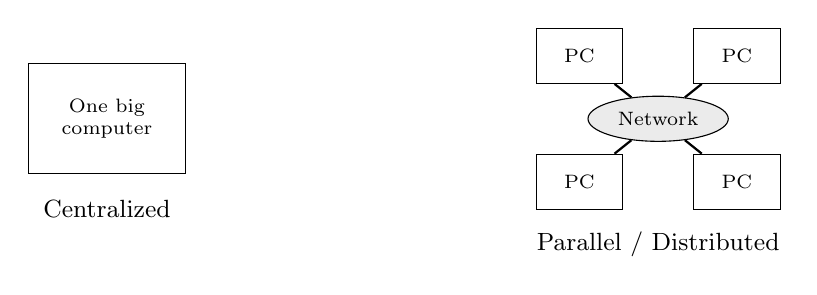
\begin{tikzpicture}[node distance=0.6cm]
\node[pc,minimum width=2cm,minimum height=1.4cm] (c) {One big\\computer};
\node[below=0.2cm of c,font=\small] {Centralized};
\node[pc] (a) at (6,0.8) {PC};
\node[pc] (b) at (8,0.8) {PC};
\node[pc] (d) at (6,-0.8) {PC};
\node[pc] (e) at (8,-0.8) {PC};
\node[draw,ellipse,font=\scriptsize,fill=black!8] (n) at (7,0) {Network};
\foreach \x in {a,b,d,e} \draw[thick] (\x)--(n);
\node[font=\small] at (7,-1.6) {Parallel / Distributed};
\end{tikzpicture}
\end{center}

\term{Machine Architecture}
{The internal design of a computer: its processor, memory, and how they are connected.}
{}

\term{Operating System (OS) Platform}
{The system software (e.g., Windows, Linux) that manages hardware and runs applications.}
{}

\term{Network Connectivity}
{How computers are linked to each other to exchange data (LAN, Internet, wireless).}
{}

\term{Application Workload}
{The amount and type of work that applications place on a computer system.}
{}

\term{Data-Intensive}
{Describes applications whose main challenge is handling very large amounts of data rather than heavy calculation.}
{Example: storing and searching billions of web pages.}

\term{Network-Centric}
{Describes computing in which the network is central; the work depends on many computers communicating.}
{}

\term{Server}
{A computer that provides data or services to other computers (clients) over a network.}
{}

%---------------------------------------------------------
\slide{22}{The Age of Internet Computing}

\term{Internet Computing}
{Computing in which services and resources are delivered over the Internet to large numbers of users.}
{}

\term{Supercomputer}
{An extremely fast computer with thousands of processors, used for very complex calculations.}
{Example: weather prediction, nuclear simulations.}

\term{Data Center}
{A large facility housing thousands of servers, storage systems, and networking equipment.}
{Companies like Google, Amazon, and Microsoft run huge data centers to provide their online services.}

\begin{center}
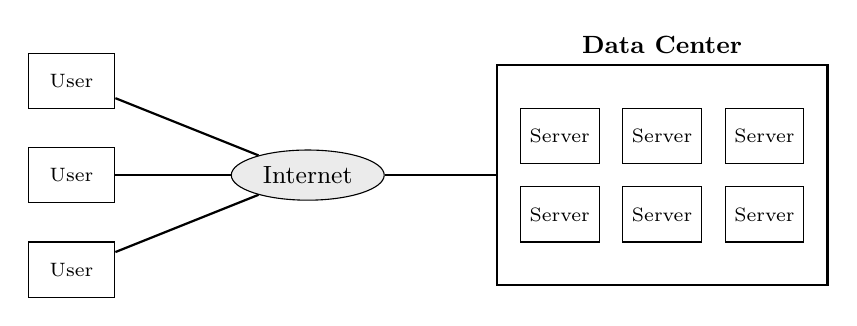
\begin{tikzpicture}
\foreach \i in {0,1,2} \node[pc] (u\i) at (0,1.2-\i*1.2) {User};
\node[draw,ellipse,fill=black!8,font=\small] (net) at (3,0) {Internet};
\node[draw,thick,minimum width=4.2cm,minimum height=2.8cm] (dc) at (7.5,0) {};
\node[font=\small\bfseries,above] at (dc.north) {Data Center};
\foreach \x in {0,1,2} \foreach \y in {0,1} \node[pc,minimum width=0.9cm] at (6.2+\x*1.3,0.5-\y*1) {Server};
\foreach \i in {0,1,2} \draw[thick] (u\i)--(net);
\draw[thick] (net)--(dc.west);
\end{tikzpicture}
\end{center}

\term{Concurrently}
{At the same time.}
{A data center serves millions of users concurrently.}

\term{Linpack Benchmark}
{A standard test program that measures how fast a computer can solve a large system of linear equations, reported in flops.}
{Used to rank the world's fastest supercomputers (Top 500 list).}

\term{Benchmark}
{A standard test used to measure and compare the performance of computers.}
{}

\term{Storage System}
{Hardware (hard disks, SSDs, storage arrays) that stores data permanently.}
{}

\term{Bandwidth}
{The maximum amount of data that can be transferred over a network per second (e.g., Gbps).}
{\textbf{High-bandwidth network} = a network that can carry a lot of data quickly.}

\term{Web Services}
{Software services offered over the web that other programs can use through standard protocols.}
{Example: a payment service used by many shopping websites.}

%---------------------------------------------------------
\slide{23}{The Platform Evolution: Five Generations}

\term{Platform}
{The type of computer hardware and system software on which applications run.}
{}

\term{Generation (of computers)}
{A stage in the history of computing marked by a major change in technology.}
{}

\begin{center}
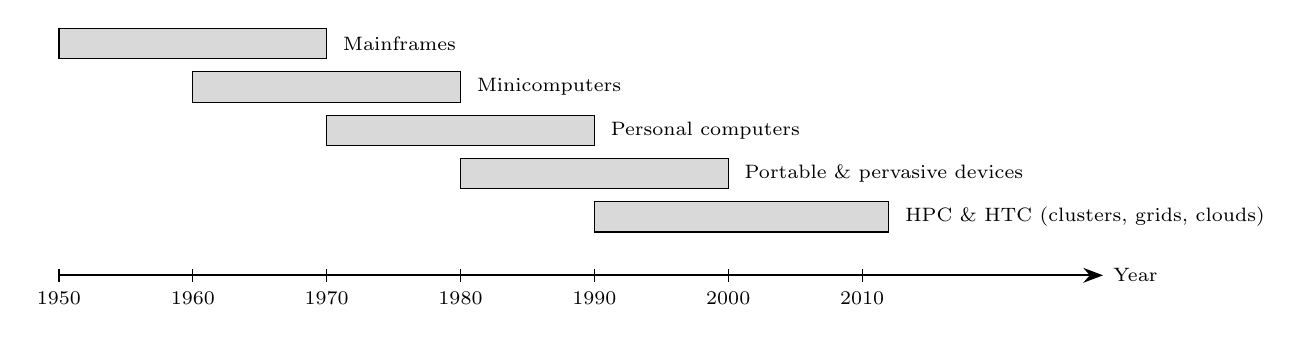
\begin{tikzpicture}[x=0.17cm,y=0.55cm]
\draw[arr] (0,0)--(78,0) node[right,font=\scriptsize]{Year};
\foreach \yr in {1950,1960,1970,1980,1990,2000,2010} {\draw ({\yr-1950},0.15)--({\yr-1950},-0.15) node[below,font=\scriptsize]{\yr};}
\foreach \s/\e/\lab/\r in {0/20/{Mainframes}/5,10/30/{Minicomputers}/4,20/40/{Personal computers}/3,30/50/{Portable \& pervasive devices}/2,40/62/{HPC \& HTC (clusters, grids, clouds)}/1}
{\fill[black!15,draw=black] (\s,\r) rectangle (\e,\r+0.7); \node[right,font=\scriptsize] at (\e+0.5,\r+0.35) {\lab};}
\end{tikzpicture}\\[-2pt]
{\footnotesize Overlapping generations of computer platforms (each 10--20 years, overlapping by about 10 years)}
\end{center}

\term{Mainframe}
{A large, powerful, expensive computer used by big organizations for bulk data processing.}
{Example: IBM 360, CDC 6400.}

\term{Minicomputer}
{A mid-sized, lower-cost computer, smaller than a mainframe.}
{Example: DEC PDP 11, VAX series; popular in small businesses and colleges.}

\term{Personal Computer (PC)}
{A computer designed for use by one person at a time.}
{}

\term{VLSI (Very Large Scale Integration)}
{The technology of placing millions (now billions) of transistors on a single chip.}
{VLSI made the microprocessor possible.}

\term{Microprocessor}
{A complete processor (CPU) built on a single chip.}
{}

\term{Portable Computer and Pervasive Device}
{Portable computers can be carried (laptops); pervasive devices are small computing devices embedded everywhere (phones, smart cards, sensors).}
{}

\term{Wired and Wireless}
{Wired: connected through cables (Ethernet); Wireless: connected through radio signals (Wi-Fi, mobile networks).}
{}

\term{Shared Web Resources}
{Computing power, storage, and software on the Internet that many users share.}
{}

%---------------------------------------------------------
\slide{24}{Evolutionary Trend toward Parallel, Distributed, and Cloud Computing}

\begin{center}
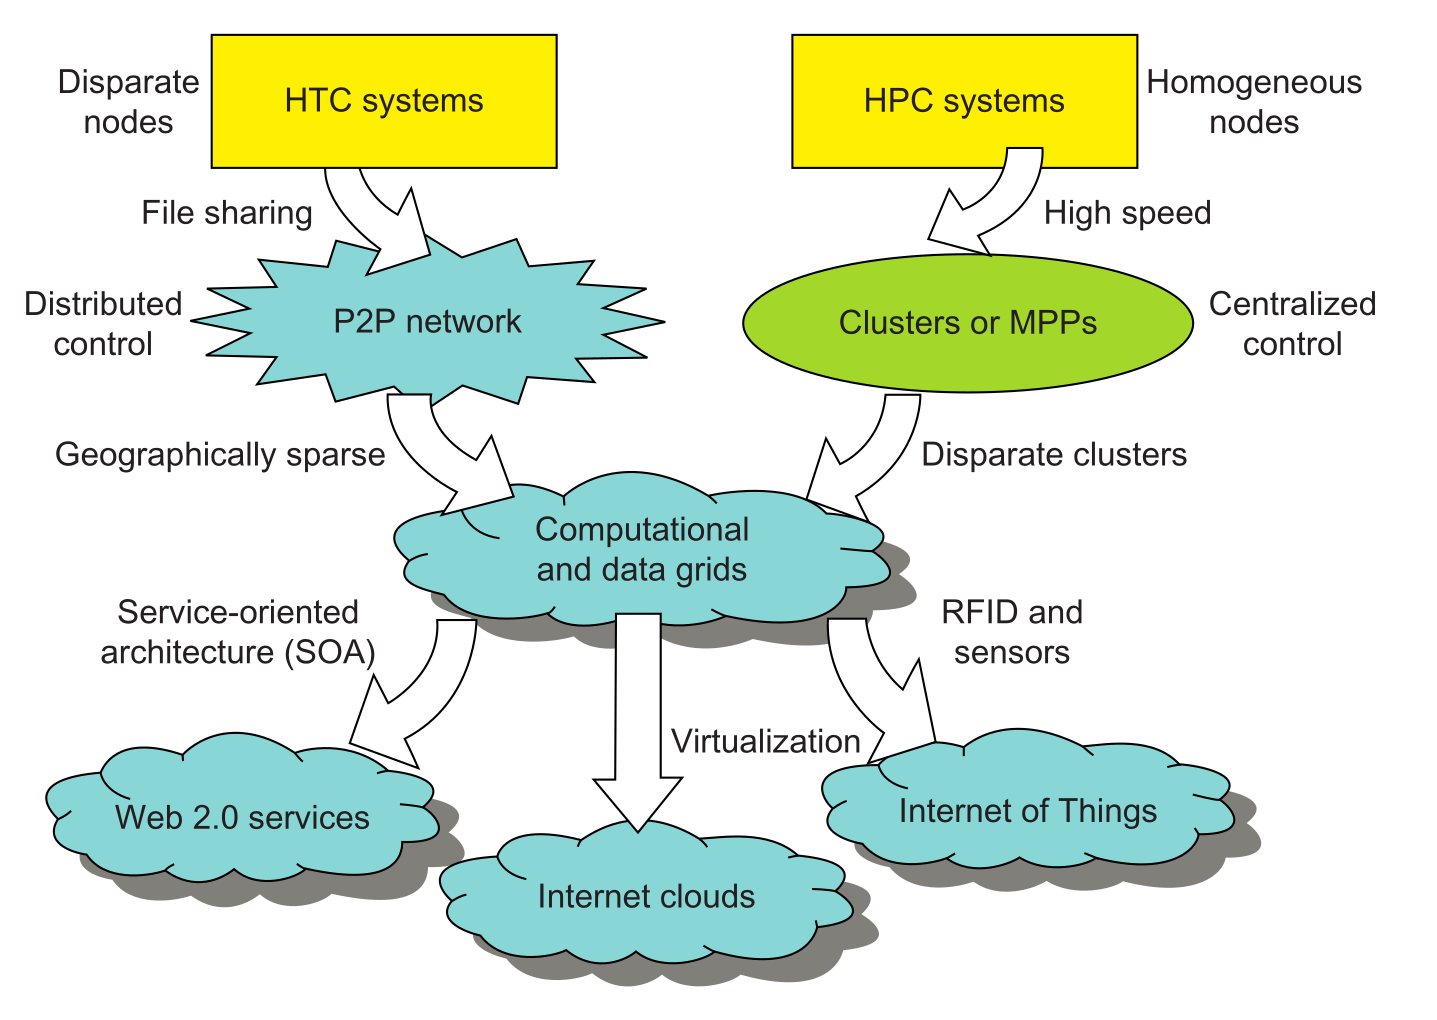
\includegraphics[width=0.55\linewidth]{images/Fig1_1_evolution_trend.png}\\
{\footnotesize Figure 1.1 of Text Book 1}
\end{center}

\term{MPP (Massively Parallel Processor)}
{A single computer with a very large number of processors working in parallel, each with its own memory, connected by a fast internal network.}
{Most traditional supercomputers are MPPs.}

\term{Cluster}
{A collection of homogeneous computers (nodes) connected closely by a fast local network and used as one system.}
{Clusters gradually replaced MPPs because they are cheaper and allow resources to be shared.}

\term{Node}
{A single computer in a cluster, grid, or network.}
{}

\term{Peer-to-Peer (P2P) Network}
{A network in which every computer (peer) acts as both client and server, sharing resources directly without a central server.}
{Example: BitTorrent file sharing.}

\begin{center}
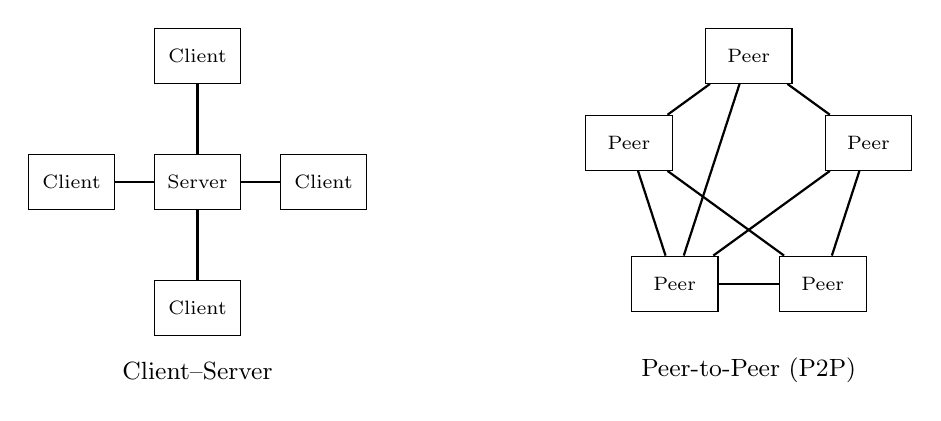
\begin{tikzpicture}
\node[pc] (s) at (0,0) {Server};
\foreach \a in {0,90,180,270} \node[pc] (c\a) at ($(s)+(\a:1.6)$) {Client};
\foreach \a in {0,90,180,270} \draw[thick] (s)--(c\a);
\node[font=\small] at (0,-2.4) {Client--Server};
\foreach \a in {90,162,234,306,18} \node[pc] (p\a) at ($(7,0)+(\a:1.6)$) {Peer};
\foreach \a/\b in {90/162,162/234,234/306,306/18,18/90,90/234,162/306,234/18} \draw[thick] (p\a)--(p\b);
\node[font=\small] at (7,-2.4) {Peer-to-Peer (P2P)};
\end{tikzpicture}
\end{center}

\term{Client}
{A computer or program that requests services from a server.}
{}

\term{Content Delivery}
{Distributing content (videos, files, web pages) to users from servers located close to them.}
{}

\term{Computational Grid and Data Grid}
{A grid connects computers from many organizations and locations to share resources. A computational grid shares processing power; a data grid shares large data sets.}
{}

\term{Web 2.0 Services}
{Interactive web applications where users create and share content.}
{Examples: social networks, blogs, wikis, online maps.}

\term{Internet Cloud}
{A pool of computing resources in large data centers offered to users over the Internet.}
{}

\term{Internet of Things (IoT)}
{A network of everyday physical objects fitted with sensors and connectivity so they can exchange data.}
{See Slide 34.}

%---------------------------------------------------------
\slide{25}{Reading Figure 1.1: Labels on the Arrows}

\term{Homogeneous Nodes}
{Computers in a system that are all of the same type (same hardware and OS).}
{Typical of clusters and MPPs.}

\term{Disparate (Heterogeneous) Nodes}
{Computers in a system that are of different types, sizes, and operating systems.}
{Typical of P2P networks and grids.}

\term{Centralized Control}
{One master computer manages and coordinates all other computers.}
{}

\term{Distributed Control}
{No single computer is in charge; decisions are shared among all computers.}
{}

\begin{center}
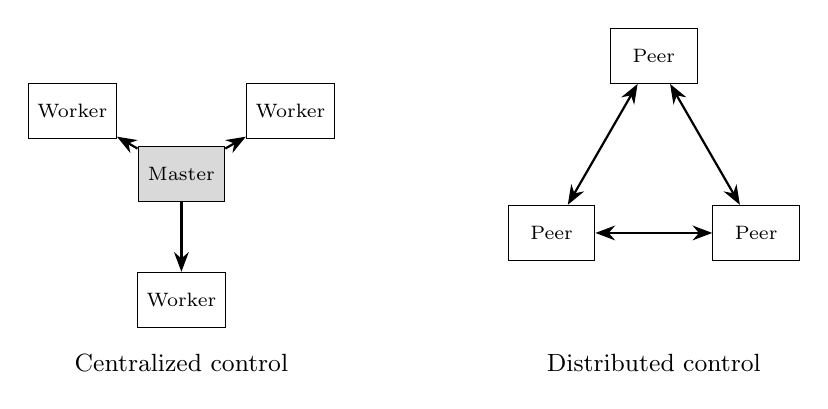
\begin{tikzpicture}
\node[pc,fill=black!15] (m) at (0,0) {Master};
\foreach \a in {30,150,270} \node[pc] (w\a) at ($(m)+(\a:1.6)$) {Worker};
\foreach \a in {30,150,270} \draw[arr] (m)--(w\a);
\node[font=\small] at (0,-2.4) {Centralized control};
\foreach \a in {90,210,330} \node[pc] (q\a) at ($(6,0)+(\a:1.5)$) {Peer};
\draw[darr] (q90)--(q210); \draw[darr] (q210)--(q330); \draw[darr] (q330)--(q90);
\node[font=\small] at (6,-2.4) {Distributed control};
\end{tikzpicture}
\end{center}

\term{Geographically Sparse}
{Spread out over a wide geographical area (different cities or countries).}
{}

\term{Disparate Clusters}
{Clusters of different types owned by different organizations.}
{When joined, they form a grid.}

\term{SOA (Service-Oriented Architecture)}
{A software design style in which applications are built from independent services that communicate over a network.}
{See Slide 29.}

\term{Virtualization}
{Technology that creates virtual (software-based) versions of computers, storage, or networks on top of real hardware.}
{See Slide 29.}

\term{RFID (Radio-Frequency Identification)}
{A technology that uses radio waves to automatically identify and track tags attached to objects.}
{Example: FASTag on vehicles for toll payment.}

\term{Sensor}
{A device that detects a physical quantity (temperature, motion, light) and converts it into data.}
{}

%---------------------------------------------------------
\slide{26}{High-Performance Computing (HPC)}

\term{High-Performance Computing (HPC)}
{The use of supercomputers and clusters to solve large, complex problems as \textbf{fast} as possible.}
{The focus is on raw speed for a single big problem.}

\term{Raw Speed Performance}
{The pure calculating speed of a computer, without considering cost or number of users.}
{}

\term{Flops (Floating-Point Operations per Second)}
{The number of calculations with decimal numbers a computer performs every second.}
{The standard unit of supercomputer speed.}

\begin{center}
\begin{tabular}{@{}llll@{}}
\toprule
\textbf{Unit} & \textbf{Prefix} & \textbf{Value} & \textbf{Era (from textbook)} \\ \midrule
Gflops & Giga & $10^{9}$ flops & Early 1990s \\
Tflops & Tera & $10^{12}$ flops & Around 2000 \\
Pflops & Peta & $10^{15}$ flops & 2010 \\ \bottomrule
\end{tabular}
\end{center}

\term{Floating-Point Number}
{A number with a decimal point, such as 3.14 or $6.02\times10^{23}$.}
{}

\term{Top 500}
{A list, updated twice a year, of the 500 most powerful computers in the world, ranked by Linpack benchmark results.}
{}

\term{Simulation}
{Using a computer model to imitate a real-world process (weather, earthquakes) to study it.}
{}

\term{Genome Analysis}
{Computer processing of DNA sequence data to study genes.}
{}

%---------------------------------------------------------
\slide{27}{High-Throughput Computing (HTC)}

\term{High-Throughput Computing (HTC)}
{Computing that aims to complete the \textbf{largest number of tasks} in a given time, rather than one task as fast as possible.}
{Suited to serving millions of independent requests, such as web searches.}

\term{Throughput}
{The number of tasks (jobs, requests) completed per unit of time.}
{Example: 10,000 search requests answered per second.}

\term{High-Flux Computing}
{Another name for HTC: computing with a very high flow (flux) of tasks passing through the system.}
{}

\term{Batch Processing}
{Running a group (batch) of jobs together without user interaction.}
{Example: generating salary slips of all employees at month end.}

\term{Reliability}
{The ability of a system to keep working correctly without failure over time.}
{}

\term{Security}
{Protection of systems and data from unauthorized access and attacks.}
{}

\term{Energy Saving}
{Reducing the electricity consumed by servers and data centers.}
{}

%---------------------------------------------------------
\slide{28}{HPC versus HTC: A Comparison}

\begin{center}
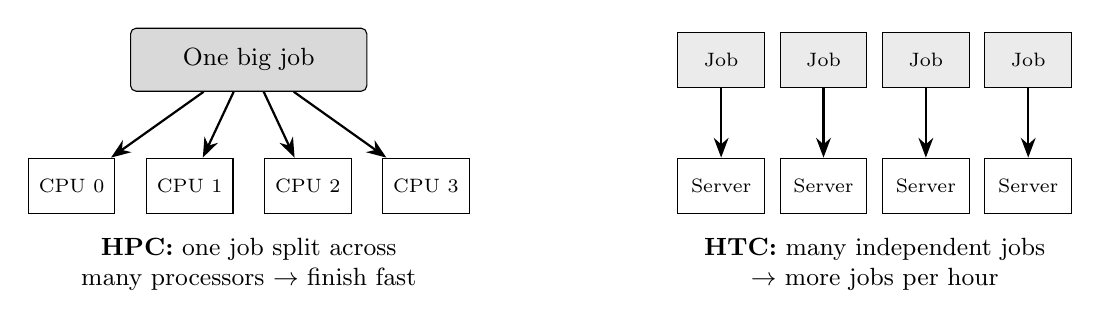
\begin{tikzpicture}
\node[box,minimum width=3cm,fill=black!15] (j) at (0,0) {One big job};
\foreach \i in {0,1,2,3} \node[pc] (p\i) at (-2.25+\i*1.5,-1.6) {CPU \i};
\foreach \i in {0,1,2,3} \draw[arr] (j)--(p\i);
\node[font=\small,align=center] at (0,-2.6) {\textbf{HPC:} one job split across\\many processors $\rightarrow$ finish fast};
\foreach \i in {0,1,2,3} {\node[pc,fill=black!8] (t\i) at (6+\i*1.3,0) {Job}; \node[pc] (s\i) at (6+\i*1.3,-1.6) {Server}; \draw[arr] (t\i)--(s\i);}
\node[font=\small,align=center] at (7.95,-2.6) {\textbf{HTC:} many independent jobs\\$\rightarrow$ more jobs per hour};
\end{tikzpicture}
\end{center}

\term{Job / Task}
{A unit of work submitted to a computer system.}
{}

\term{Analogy: Racing Car vs Metro Train}
{HPC is like a racing car: it carries one passenger very fast. HTC is like a metro train: each trip is not the fastest, but it carries thousands of passengers per hour.}
{}

%---------------------------------------------------------
\slide{29}{Three New Computing Paradigms}

\term{Service-Oriented Architecture (SOA)}
{A way of building software as a collection of independent \textbf{services}, each doing one job, that communicate over a network using standard interfaces.}
{A service provider publishes its service in a registry; a service consumer finds it and uses it.}

\begin{center}
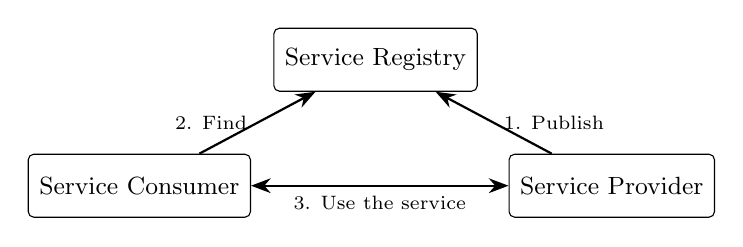
\begin{tikzpicture}
\node[box] (r) at (3,1.6) {Service Registry};
\node[box] (p) at (6,0) {Service Provider};
\node[box] (c) at (0,0) {Service Consumer};
\draw[arr] (p)--node[right,font=\scriptsize]{1. Publish} (r);
\draw[arr] (c)--node[left,font=\scriptsize]{2. Find} (r);
\draw[darr] (c)--node[below,font=\scriptsize]{3. Use the service} (p);
\end{tikzpicture}
\end{center}

\term{Virtualization}
{Creating several virtual machines (VMs) on one physical computer using software called a \textbf{hypervisor}; each VM behaves like a separate computer with its own OS.}
{Virtualization is the key technology behind cloud computing.}

\begin{center}
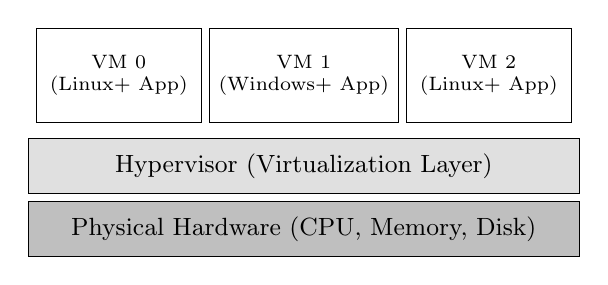
\begin{tikzpicture}
\node[draw,minimum width=7cm,minimum height=0.7cm,fill=black!25,font=\small] (hw) at (0,0) {Physical Hardware (CPU, Memory, Disk)};
\node[draw,minimum width=7cm,minimum height=0.7cm,fill=black!12,font=\small] (hv) at (0,0.8) {Hypervisor (Virtualization Layer)};
\foreach \i/\os in {0/Linux,1/Windows,2/Linux} {\node[draw,minimum width=2.1cm,minimum height=1.2cm,font=\scriptsize,align=center] at (-2.35+\i*2.35,1.95) {VM \i\\(\os + App)};}
\end{tikzpicture}
\end{center}

\term{Virtual Machine (VM)}
{A software-based computer that runs on a physical machine and behaves like a real computer.}
{}

\term{GPS (Global Positioning System)}
{A satellite-based system that gives the exact location of a receiver anywhere on Earth.}
{}

\term{Paradigms Blurring}
{The boundaries between clusters, grids, P2P systems, and clouds are becoming less clear, since clouds are often built from clusters with virtualization added.}
{}

%---------------------------------------------------------
\slide{30}{How the Idea of a ``Computer'' Has Changed}

\term{Computer Utility}
{The idea that computing can be supplied to homes and offices like a public utility (electricity, water, telephone).}
{Predicted by Leonard Kleinrock in 1969; realized today by cloud computing.}

\term{``The Network is the Computer''}
{John Gage's (Sun Microsystems, 1984) idea that the real power lies in many networked computers, not in one machine.}
{}

\term{``The Data Center is the Computer''}
{David Patterson's (2008) idea that an entire data center should be designed and programmed as one giant computer.}
{}

\term{``The Cloud is the Computer''}
{Rajkumar Buyya's idea that users simply use the cloud, without caring which physical machine does the work.}
{}

\term{Software as a Service}
{Software that runs on the provider's servers and is used through the Internet instead of being installed on the user's PC.}
{Example: Google Docs versus installing a word processor.}

%---------------------------------------------------------
\slide{31}{Computing Paradigm Distinctions (1/2)}

\term{Centralized Computing}
{A paradigm in which all computer resources --- processors, memory, and storage --- are in one physical system, fully shared and controlled by one operating system.}
{}

\term{Tightly Coupled}
{Components that are closely connected and depend heavily on each other, typically sharing memory.}
{}

\term{Loosely Coupled}
{Components that are connected but work fairly independently, each with its own memory.}
{}

\term{Integrated OS}
{A single operating system that manages all resources of the system.}
{}

\term{Parallel Computing (Parallel Processing)}
{Using many processors at the same time to solve one problem faster by dividing it into parts.}
{}

\term{Shared Memory}
{One memory that all processors can read and write directly.}
{Processors communicate by writing to and reading from common memory locations.}

\term{Distributed Memory}
{Each processor has its own private memory; processors communicate by sending messages.}
{}

\begin{center}
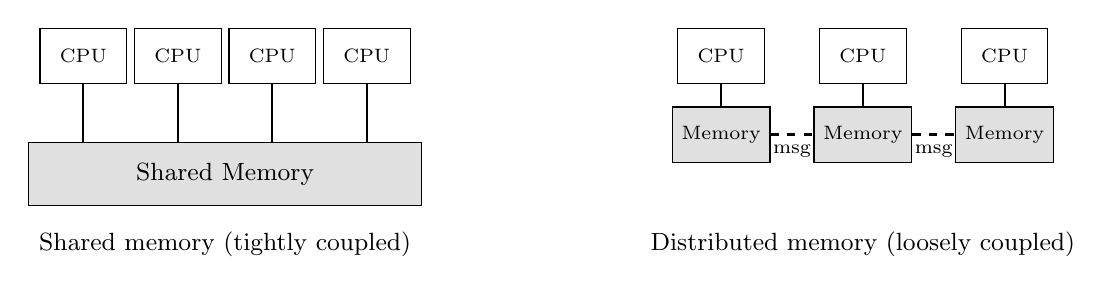
\begin{tikzpicture}
\node[draw,minimum width=5cm,minimum height=0.8cm,fill=black!12,font=\small] (sm) at (0,0) {Shared Memory};
\foreach \i in {0,1,2,3} {\node[pc] (c\i) at (-1.8+\i*1.2,1.5) {CPU}; \draw[thick] (c\i)--(c\i|-sm.north);}
\node[font=\small] at (0,-0.9) {Shared memory (tightly coupled)};
\foreach \i in {0,1,2} {\node[pc] (d\i) at (6.3+\i*1.8,1.5) {CPU}; \node[pc,fill=black!12] (m\i) at (6.3+\i*1.8,0.5) {Memory}; \draw[thick] (d\i)--(m\i);}
\draw[thick,dashed] (m0)--(m1) node[midway,below,font=\scriptsize]{msg}; \draw[thick,dashed] (m1)--(m2) node[midway,below,font=\scriptsize]{msg};
\node[font=\small] at (8.1,-0.9) {Distributed memory (loosely coupled)};
\end{tikzpicture}
\end{center}

\term{Interprocessor Communication}
{The exchange of data between processors working on the same problem.}
{}

\term{Message Passing}
{A method of communication in which processes exchange data by explicitly sending and receiving messages.}
{}

\term{Parallel Computer, Parallel Program, Parallel Programming}
{A parallel computer can run many computations at once; a parallel program is software written for it; parallel programming is the process of writing such programs.}
{}

%---------------------------------------------------------
\slide{32}{Computing Paradigm Distinctions (2/2)}

\term{Distributed Computing}
{The field of computer science that studies distributed systems.}
{}

\term{Distributed System}
{A system of multiple \textbf{autonomous} computers, each with its own private memory, that communicate through a computer network and work together.}
{To the user, the whole system appears as one.}

\term{Autonomous Computer}
{A computer that is independent: it has its own processor, memory, and OS and can work on its own.}
{}

\term{Distributed Program and Distributed Programming}
{A distributed program runs across many computers in a distributed system; writing such programs is distributed programming.}
{}

\term{Cloud Computing}
{A paradigm in which a pool of physical or virtualized resources in large data centers is offered to users over the Internet, using parallel and/or distributed computing.}
{Users pay only for what they use and need not own the hardware.}

\begin{center}
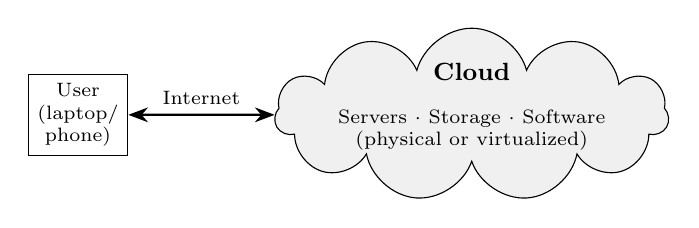
\begin{tikzpicture}
\node[pc] (u) at (0,0) {User\\(laptop/\\phone)};
\node[draw,cloud,cloud puffs=11,aspect=2.2,minimum width=5cm,minimum height=2.2cm,fill=black!6] (cl) at (5,0) {};
\node[font=\small\bfseries] at (5,0.55) {Cloud};
\node[font=\scriptsize,align=center] at (5,-0.2) {Servers $\cdot$ Storage $\cdot$ Software\\(physical or virtualized)};
\draw[darr] (u)--node[above,font=\scriptsize]{Internet} (cl.west);
\end{tikzpicture}
\end{center}

\term{Physical vs Virtualized Resources}
{Physical resources are real hardware; virtualized resources are software-created versions (VMs) running on that hardware.}
{}

\term{Service Computing}
{Computing in which everything is offered and used as a service over the network.}
{}

%---------------------------------------------------------
\slide{33}{Computing Paradigms at a Glance}

\term{Overlap of Paradigms}
{The paradigms are not completely separate: parallel computing overlaps with distributed computing, and cloud computing uses ideas from centralized, parallel, and distributed computing.}
{}

\begin{center}
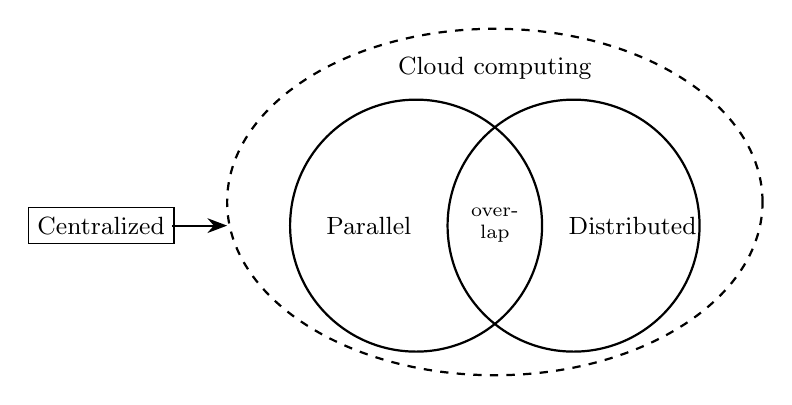
\begin{tikzpicture}
\draw[thick] (0,0) circle (1.6); \node[font=\small] at (-0.6,0) {Parallel};
\draw[thick] (2,0) circle (1.6); \node[font=\small] at (2.75,0) {Distributed};
\node[font=\scriptsize,align=center] at (1,0) {over-\\lap};
\draw[thick,dashed] (1,0.3) ellipse (3.4 and 2.2);
\node[font=\small] at (1,2.0) {Cloud computing};
\node[draw,font=\small] at (-4,0) {Centralized};
\draw[arr] (-3.1,0)--(-2.4,0);
\end{tikzpicture}\\
{\footnotesize Distributed computing is the opposite of centralized computing; the paradigms overlap.}
\end{center}

\term{Opposite of Centralized}
{Distributed computing spreads resources over many computers, whereas centralized computing keeps them in one system.}
{}

%---------------------------------------------------------
\slide{34}{Related Terms}

\term{Concurrent Computing / Concurrent Programming}
{Executing several computations during overlapping time periods; usually refers to the union of parallel and distributed computing.}
{}

\term{Ubiquitous Computing}
{Computing that is available everywhere and at any time, using small pervasive devices with wired or wireless communication.}
{Example: smartphones, smart watches, smart home devices.}

\term{Pervasive Device}
{A small computing device embedded in everyday surroundings.}
{}

\term{Internet of Things (IoT)}
{A networked connection of everyday objects --- computers, sensors, machines, even humans --- that collect and exchange data, supported by Internet clouds.}
{}

\begin{center}
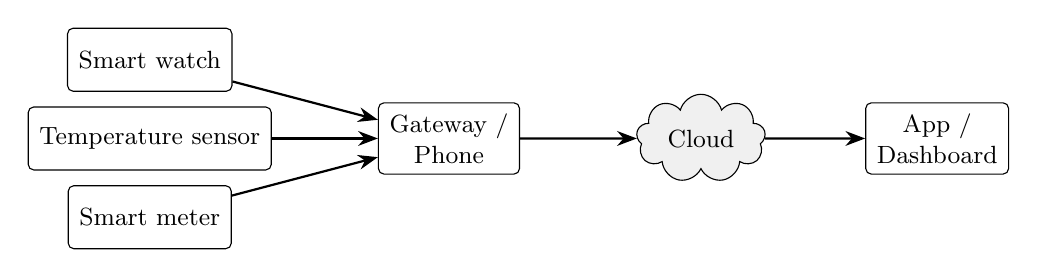
\begin{tikzpicture}
\node[box] (s1) at (0,1) {Smart watch};
\node[box] (s2) at (0,0) {Temperature sensor};
\node[box] (s3) at (0,-1) {Smart meter};
\node[box] (g) at (3.8,0) {Gateway /\\Phone};
\node[draw,cloud,cloud puffs=9,aspect=2,fill=black!6,font=\small] (c) at (7,0) {Cloud};
\node[box] (a) at (10,0) {App /\\Dashboard};
\foreach \i in {1,2,3} \draw[arr] (s\i)--(g);
\draw[arr] (g)--(c); \draw[arr] (c)--(a);
\end{tikzpicture}
\end{center}

\term{Internet Computing}
{The broadest term, covering all computing paradigms over the Internet.}
{}

%---------------------------------------------------------
\slide{35}{Distributed System Families}

\term{Distributed System Family}
{A group of related distributed system types: clusters, grids, P2P networks, and clouds.}
{}

\term{Wide Area Computing Infrastructure}
{Computing facilities connected across a large geographical area (a country or the world).}
{}

\term{Grid (Computational / Data Grid)}
{A system that connects clusters and computers owned by different organizations across many locations so they can share computing power and data.}
{}

\begin{center}
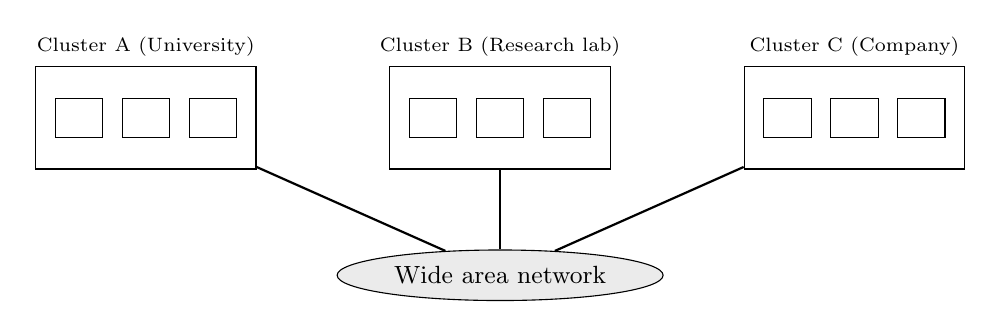
\begin{tikzpicture}
\foreach \i/\lab/\x in {0/{Cluster A (University)}/0,1/{Cluster B (Research lab)}/4.5,2/{Cluster C (Company)}/9} {
  \node[draw,minimum width=2.8cm,minimum height=1.3cm] (k\i) at (\x,0) {};
  \node[font=\scriptsize,above] at (k\i.north) {\lab};
  \foreach \j in {0,1,2} \node[pc,minimum width=0.6cm,minimum height=0.5cm] at (\x-0.85+\j*0.85,0) {};
}
\node[draw,ellipse,fill=black!8,font=\small] (w) at (4.5,-2) {Wide area network};
\foreach \i in {0,1,2} \draw[thick] (k\i)--(w);
\end{tikzpicture}\\
{\footnotesize A grid joins clusters owned by different organizations over a wide area network.}
\end{center}

\term{Service-Oriented Computing}
{Computing in which software functions are provided as services over a network.}
{}

\term{Resource Sharing}
{Allowing many users or organizations to use the same hardware, software, and data.}
{}

\term{Massively Distributed System}
{A distributed system made of a very large number (thousands to millions) of machines.}
{}

\term{Parallelism / Concurrency}
{Parallelism: doing many things at exactly the same time on different processors. Concurrency: managing many tasks in overlapping time.}
{}

\term{CPU Core}
{An individual processing unit inside a CPU; a multicore CPU has several cores.}
{}

\term{GPU (Graphics Processing Unit)}
{A processor with thousands of small cores, originally for graphics, now used for fast parallel calculations.}
{Tianhe-1A had over 3.2 million GPU cores.}

\term{Tianhe-1A}
{A Chinese supercomputer that was the fastest cluster machine in the world in October 2010.}
{}

%---------------------------------------------------------
\slide{36}{Design Objectives for Future HPC and HTC Systems}

\term{Multicore / Many-core Processor}
{A processor chip with several (multicore) or very many (many-core) processing cores.}
{}

\term{Thread}
{The smallest sequence of instructions that can be scheduled and run independently by a processor.}
{A program can have many threads running at once.}

\term{Throughput per Watt}
{The amount of work done for each unit of electrical power consumed; a measure of energy efficiency.}
{}

\term{Efficiency}
{How well a system uses its resources (processors, memory, power) to get work done.}
{}

\term{Utilization Rate}
{The fraction of time a resource is actually busy doing useful work.}
{}

\term{Dependability}
{The ability of a system to deliver service that can be trusted --- reliable, available, and self-managing --- even when parts fail.}
{}

\term{Self-Management}
{The ability of a system to monitor, configure, and repair itself automatically.}
{}

\term{Quality of Service (QoS)}
{A guaranteed level of performance, such as response time, availability, and throughput.}
{}

\term{Programming Model}
{The way a programmer is expected to write programs for a system (e.g., parallel or distributed programming model).}
{}

\term{Adaptation}
{The ability of the programming model to handle huge numbers of requests and data sets on virtualized cloud resources.}
{}

\term{Flexibility in Application Deployment}
{The ability of a system to run both scientific (HPC) and business (HTC) applications well.}
{}

\term{Deployment}
{Installing and running an application on a system so that users can use it.}
{}

%---------------------------------------------------------
\slide{37}{Scalable Computing Trends}

\term{Rules of Thumb in Data Engineering}
{A well-known paper by Jim Gray describing practical trends in storage, processing, and networking costs.}
{}

\term{Moore's Law}
{The observation that processor speed (originally, the number of transistors on a chip) doubles roughly every 18 months.}
{}

\begin{center}
\begin{tikzpicture}[x=0.6cm,y=0.07cm]
\draw[arr] (0,0)--(10.5,0) node[right,font=\scriptsize]{Years};
\draw[arr] (0,0)--(0,72) node[above,font=\scriptsize]{Relative speed};
\draw[very thick,domain=0:9,samples=60] plot (\x,{2^(\x/1.5)});
\foreach \t/\v in {0/1,1.5/2,3/4,4.5/8,6/16,7.5/32,9/64} {\fill (\t,{\v}) circle (1.5pt); \node[left,font=\tiny] at (\t,{\v+2}) {$\times$\v};}
\foreach \t in {0,3,6,9} \node[below,font=\scriptsize] at (\t,0) {\t};
\end{tikzpicture}\\
{\footnotesize Moore's law: doubling every 1.5 years gives 64 times the speed in 9 years.}
\end{center}

\term{Gilder's Law}
{The observation that network bandwidth has doubled every year.}
{}

\term{Commodity Hardware}
{Ordinary, mass-produced, low-cost computer components (like those in desktops and laptops).}
{Large clusters and data centers are built from commodity hardware because it is cheap.}

\term{Price/Performance Ratio}
{The cost of a system divided by its performance; a lower value means better value for money.}
{}

\term{Degree of Parallelism (DoP)}
{The number of operations or tasks that can be executed at the same time.}
{}

\term{Resource Distribution}
{Spreading computing resources across many machines and locations.}
{}

%---------------------------------------------------------
\slide{38}{Degrees of Parallelism}

\term{Bit-Serial Processing}
{Processing data one bit at a time.}
{}

\term{Bit-Level Parallelism (BLP)}
{Processing many bits at once by increasing the word size of the processor (4 $\rightarrow$ 8 $\rightarrow$ 16 $\rightarrow$ 32 $\rightarrow$ 64 bits).}
{}

\term{Word}
{The number of bits a processor handles as one unit (e.g., 64 bits on modern CPUs).}
{}

\term{Instruction-Level Parallelism (ILP)}
{Executing several machine instructions of a program at the same time inside one processor.}
{}

\term{Pipelining}
{Splitting instruction execution into stages (fetch, decode, execute) so that different instructions are in different stages at the same time, like an assembly line.}
{}

\begin{center}
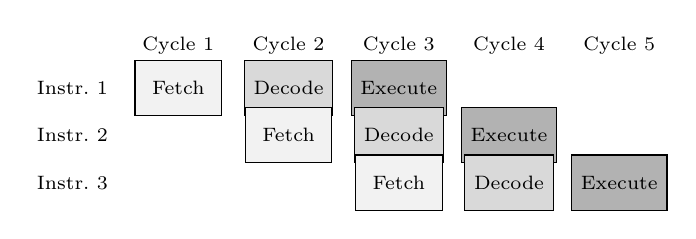
\begin{tikzpicture}[x=1.4cm,y=0.6cm]
\foreach \c in {1,...,5} \node[font=\scriptsize] at (\c,0.9) {Cycle \c};
\foreach \i/\s in {1/1,2/2,3/3} {
  \node[font=\scriptsize,anchor=east] at (0.45,-\i+1) {Instr.\ \i};
  \node[pc,fill=black!5] at (\s,-\i+1) {Fetch};
  \node[pc,fill=black!15] at (\s+1,-\i+1) {Decode};
  \node[pc,fill=black!30] at (\s+2,-\i+1) {Execute};}
\end{tikzpicture}\\
{\footnotesize Pipelining: in cycle 3, three instructions are being processed at once.}
\end{center}

\term{Superscalar Processor}
{A processor that can issue and execute more than one instruction per clock cycle using multiple execution units.}
{}

\term{VLIW (Very Long Instruction Word)}
{An architecture in which the compiler packs several independent operations into one long instruction that executes in parallel.}
{}

\term{Multithreading}
{Running multiple threads on a processor so that its resources are kept busy.}
{}

\term{Branch Prediction, Dynamic Scheduling, Speculation}
{Techniques that help ILP: guessing the outcome of \texttt{if} decisions in advance, reordering instructions at run time, and executing instructions before it is certain they are needed.}
{}

\term{Compiler}
{A program that translates source code written by a programmer into machine instructions.}
{}

\term{Data-Level Parallelism (DLP)}
{Applying the same operation to many data items at the same time.}
{}

\term{SIMD (Single Instruction, Multiple Data)}
{A processor design in which one instruction operates on many data elements simultaneously.}
{}

\begin{center}
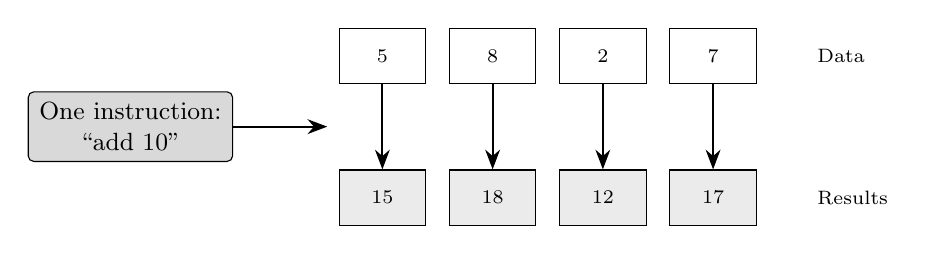
\begin{tikzpicture}
\node[box,fill=black!15] (ins) at (0,0) {One instruction:\\ ``add 10''};
\foreach \i/\d in {0/5,1/8,2/2,3/7} {\node[pc] (d\i) at (3.2+\i*1.4,0.9) {\d}; \node[pc,fill=black!8] (r\i) at (3.2+\i*1.4,-0.9) {\the\numexpr\d+10\relax}; \draw[arr] (d\i)--(r\i);}
\draw[arr] (ins)--(2.5,0);
\node[font=\scriptsize,anchor=west] at (8.6,0.9) {Data};
\node[font=\scriptsize,anchor=west] at (8.6,-0.9) {Results};
\end{tikzpicture}\\
{\footnotesize SIMD: one instruction processes four data items at the same time.}
\end{center}

\term{Vector Machine}
{A processor whose instructions work on whole arrays (vectors) of numbers at once.}
{}

\term{Task-Level Parallelism (TLP)}
{Running different tasks (parts of a program) on different cores at the same time.}
{}

\term{Chip Multiprocessor (CMP)}
{A single chip containing multiple processor cores (a multicore processor).}
{}

\term{Job-Level Parallelism (JLP)}
{Running entire independent jobs on different computers at the same time in a distributed system.}
{}

\term{Granularity (Fine-grain vs Coarse-grain)}
{The size of the work units executed in parallel. Fine-grain: small units such as bits and instructions; coarse-grain: large units such as tasks and jobs.}
{}

\begin{center}
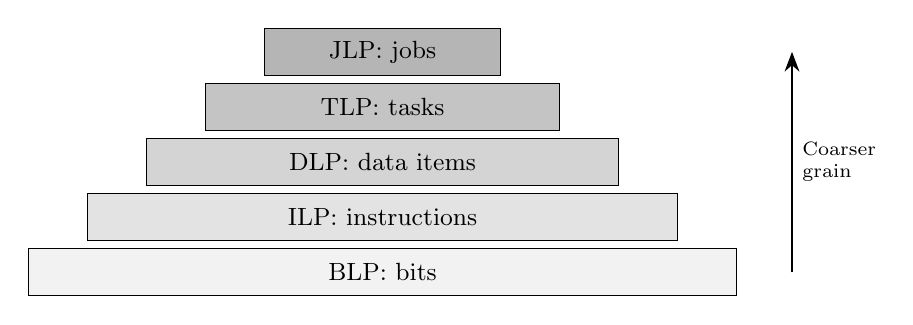
\begin{tikzpicture}
\foreach \i/\lab/\w in {0/BLP: bits/9,1/ILP: instructions/7.5,2/DLP: data items/6,3/TLP: tasks/4.5,4/JLP: jobs/3} {
\node[draw,minimum width=\w cm,minimum height=0.6cm,fill=black!\the\numexpr 5+\i*6\relax,font=\small] at (0,\i*0.7) {\lab};}
\draw[arr] (5.2,0)--(5.2,2.8) node[midway,right,font=\scriptsize,align=left]{Coarser\\grain};
\end{tikzpicture}\\
{\footnotesize Coarse-grain parallelism is built on top of fine-grain parallelism.}
\end{center}

%---------------------------------------------------------
\slide{39}{Degrees of Parallelism: An Everyday View}

\term{Pixel}
{The smallest dot of colour in a digital image.}
{Brightening every pixel of a photo with one instruction is an example of DLP.}

\term{Assembly Line}
{A production method in which a product moves through stations, each doing one step; used as an analogy for pipelining (ILP).}
{}

\term{Parallel Processing vs Distributed Processing}
{Parallel processing happens inside one computer (many processors/cores); distributed processing happens across many computers on a network.}
{Granularity increases from parallel to distributed processing.}

%---------------------------------------------------------
\slide{40}{Innovative Applications}

\term{Telecommunication}
{Communication over a distance using electronic means (telephone, mobile, Internet).}
{}

\term{E-commerce}
{Buying and selling goods and services over the Internet.}
{}

\term{Transaction Processing}
{Handling business operations (transactions) such as payments and bookings so that each is completed fully and correctly.}
{}

\term{Telemedicine}
{Providing medical consultation and care remotely using telecommunication technology.}
{}

\term{Distance Education}
{Teaching students who are not physically present, using online platforms.}
{}

\term{Electric Power Grid}
{The network that delivers electricity from power plants to consumers; it is monitored and controlled by computers.}
{}

\term{Decision-Making System}
{A computer system that analyzes data to help people make decisions.}
{}

\term{Worm Containment}
{Detecting and stopping the spread of computer worms (self-copying malicious programs) across networks.}
{}

\term{Cyber Security}
{Protecting computers, networks, and data from digital attacks.}
{}

\term{Digital Government (e-Governance)}
{Delivering government services online.}
{Example: online income tax return filing.}

\term{Mission-Critical Application}
{An application whose failure can cause serious loss of life, money, or security.}
{Examples: military command and control, crisis management.}

\term{Intelligent System}
{A computer system that can learn, reason, or adapt using AI techniques.}
{}

%---------------------------------------------------------
\slide{41}{Requirements of Innovative Applications}

\term{Transparency}
{Hiding the complexity of a distributed system so that users see it as one simple system.}
{}

\begin{center}
\renewcommand{\arraystretch}{1.25}
\small
\begin{tabularx}{\linewidth}{@{}lX@{}}
\toprule
\textbf{Type of Transparency} & \textbf{The user does not need to know\ldots} \\ \midrule
Data access & where or how the data is stored \\
Resource allocation & which machines are given to the job \\
Process location & on which computer the program is running \\
Concurrency & that many other users are running jobs at the same time \\
Job replication & that copies of the job are running for safety \\
Failure recovery & that a machine failed and the system recovered \\ \bottomrule
\end{tabularx}
\end{center}

\term{Resource Allocation}
{Assigning processors, memory, and storage to jobs.}
{}

\term{Replication}
{Keeping copies of data or jobs on multiple machines for reliability and speed.}
{}

\term{Failure Recovery}
{Restoring normal operation automatically after a hardware or software failure.}
{}

\term{Computing Economics}
{Achieving the required computing at the lowest possible cost.}
{}

\term{Web-Scale Data Collection}
{Collecting data from the entire web or from millions of users.}
{}

\term{Scalable Performance}
{Performance that grows in proportion as more resources are added.}
{}

\term{Distributed Transaction}
{A transaction that updates data stored on two or more database servers; it must succeed on all of them or on none.}
{}

\term{Database Server}
{A server that stores and manages a database and answers queries.}
{}

\term{Consistency of Replicated Records}
{Ensuring that all copies of the same data on different servers have the same value at all times.}
{}

\begin{center}
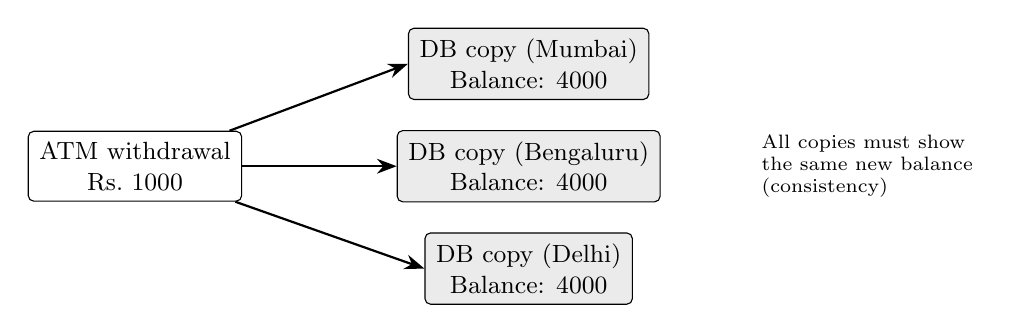
\begin{tikzpicture}
\node[box] (u) at (0,0) {ATM withdrawal\\Rs.\ 1000};
\foreach \i/\c in {0/Mumbai,1/Bengaluru,2/Delhi} \node[box,fill=black!8] (db\i) at (5,1.3-\i*1.3) {DB copy (\c)\\Balance: 4000};
\foreach \i in {0,1,2} \draw[arr] (u)--(db\i.west);
\node[font=\scriptsize,align=left] at (9.3,0) {All copies must show\\the same new balance\\(consistency)};
\end{tikzpicture}
\end{center}

\term{Network Saturation}
{A condition in which a network is so full of traffic that it cannot carry more data, causing delays.}
{}

\term{Security Threat}
{Any possible danger that can exploit a weakness to harm a system (hacking, viruses, data theft).}
{}

%---------------------------------------------------------
\slide{42}{The Trend toward Utility Computing}

\begin{center}
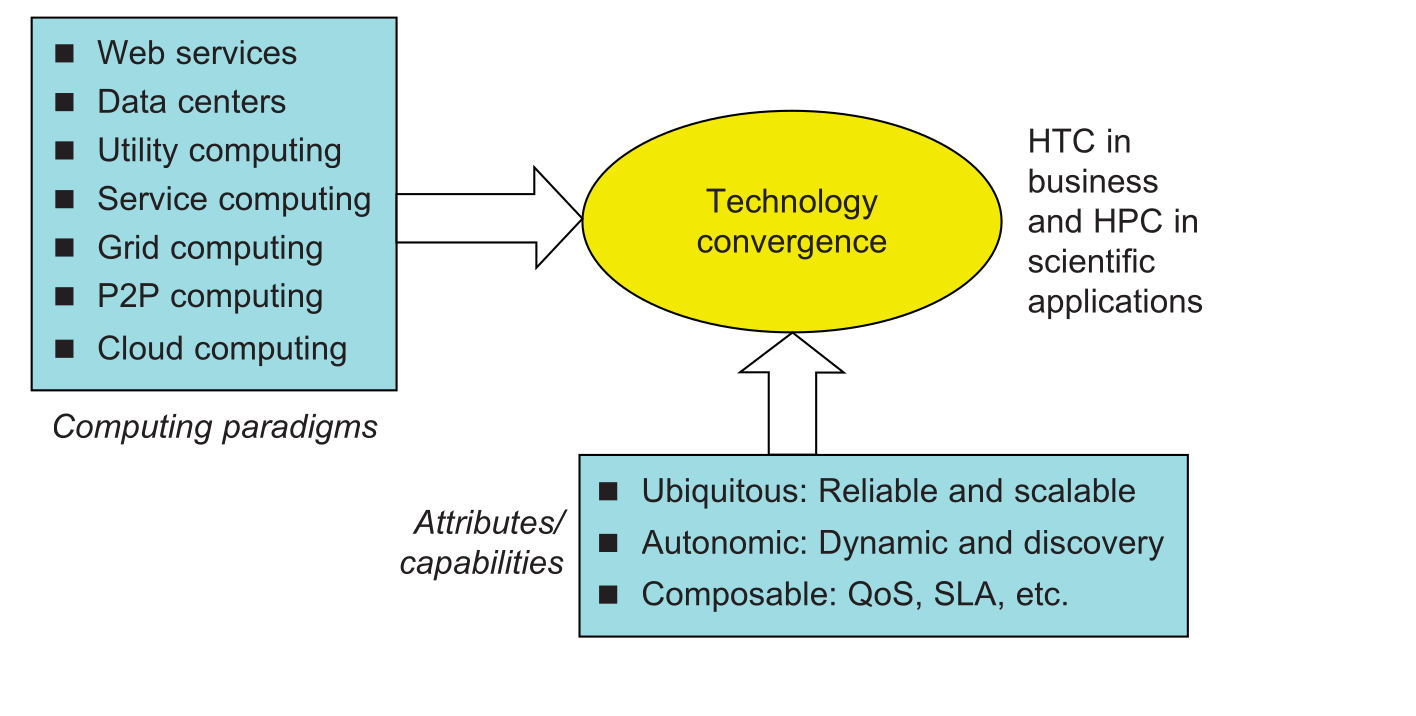
\includegraphics[width=0.6\linewidth]{images/Fig1_2_computer_utilities.png}\\
{\footnotesize Figure 1.2 of Text Book 1}
\end{center}

\term{Service Computing}
{Computing in which applications are composed from services offered over the network.}
{}

\term{P2P Computing}
{Computing performed by peers that share resources directly with each other.}
{}

\term{Technology Convergence}
{Different technologies coming together and merging into a common platform.}
{All the computing paradigms in Figure 1.2 converge to support HTC in business and HPC in science.}

%---------------------------------------------------------
\slide{43}{Common Characteristics of These Paradigms}

\term{Ubiquitous}
{Present everywhere in daily life.}
{Requires the systems to be \textbf{reliable} and \textbf{scalable}.}

\term{Scalability}
{The ability of a system to handle more work by adding more resources without a drop in performance.}
{}

\term{Autonomic}
{Able to manage itself automatically --- configuring, healing, and organizing --- without human intervention.}
{}

\term{Self-Organization}
{The ability of a system to arrange and reorganize its components automatically.}
{}

\term{Dynamic Discovery}
{Automatically finding available resources or services at run time.}
{}

\term{Composable}
{Able to be combined with other services to build larger applications.}
{}

\term{SLA (Service-Level Agreement)}
{A formal contract between a service provider and a customer that specifies the level of service guaranteed (e.g., 99.9\% availability) and penalties if not met.}
{}

%---------------------------------------------------------
\slide{44}{Utility Computing}

\term{Utility Computing}
{A business model in which customers obtain computing resources from a paid service provider and pay according to usage.}
{Like an electricity meter: you pay for the units you consume.}

\begin{center}
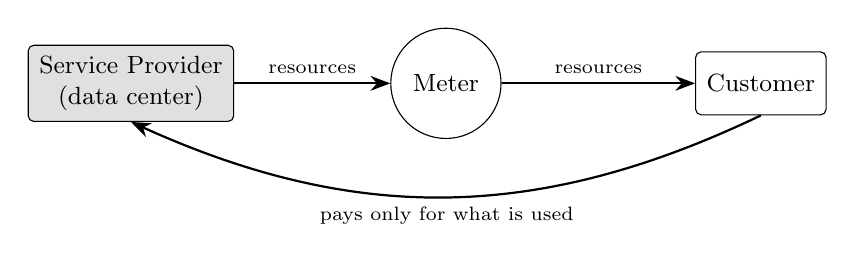
\begin{tikzpicture}
\node[box,fill=black!12] (p) at (0,0) {Service Provider\\(data center)};
\node[draw,circle,font=\small,minimum size=1.4cm] (m) at (4,0) {Meter};
\node[box] (c) at (8,0) {Customer};
\draw[arr] (p)--node[above,font=\scriptsize]{resources} (m);
\draw[arr] (m)--node[above,font=\scriptsize]{resources} (c);
\draw[arr] (c.south) to[bend left=25] node[below,font=\scriptsize]{pays only for what is used} (p.south);
\end{tikzpicture}
\end{center}

\term{Service Provider}
{A company that offers computing resources or services to customers.}
{Examples: Amazon Web Services, Microsoft Azure, Google Cloud.}

\term{Edge Network}
{The part of a network close to the end users and devices.}
{}

\term{Distributed OS}
{An operating system that manages a group of networked computers and makes them appear as one system.}
{}

\term{Middleware}
{Software that sits between the operating system and applications, connecting distributed components.}
{}

\term{Resource Management}
{Allocating, scheduling, and monitoring computing resources efficiently.}
{}

%---------------------------------------------------------
\slide{45}{The Hype Cycle of New Technologies}

\begin{center}
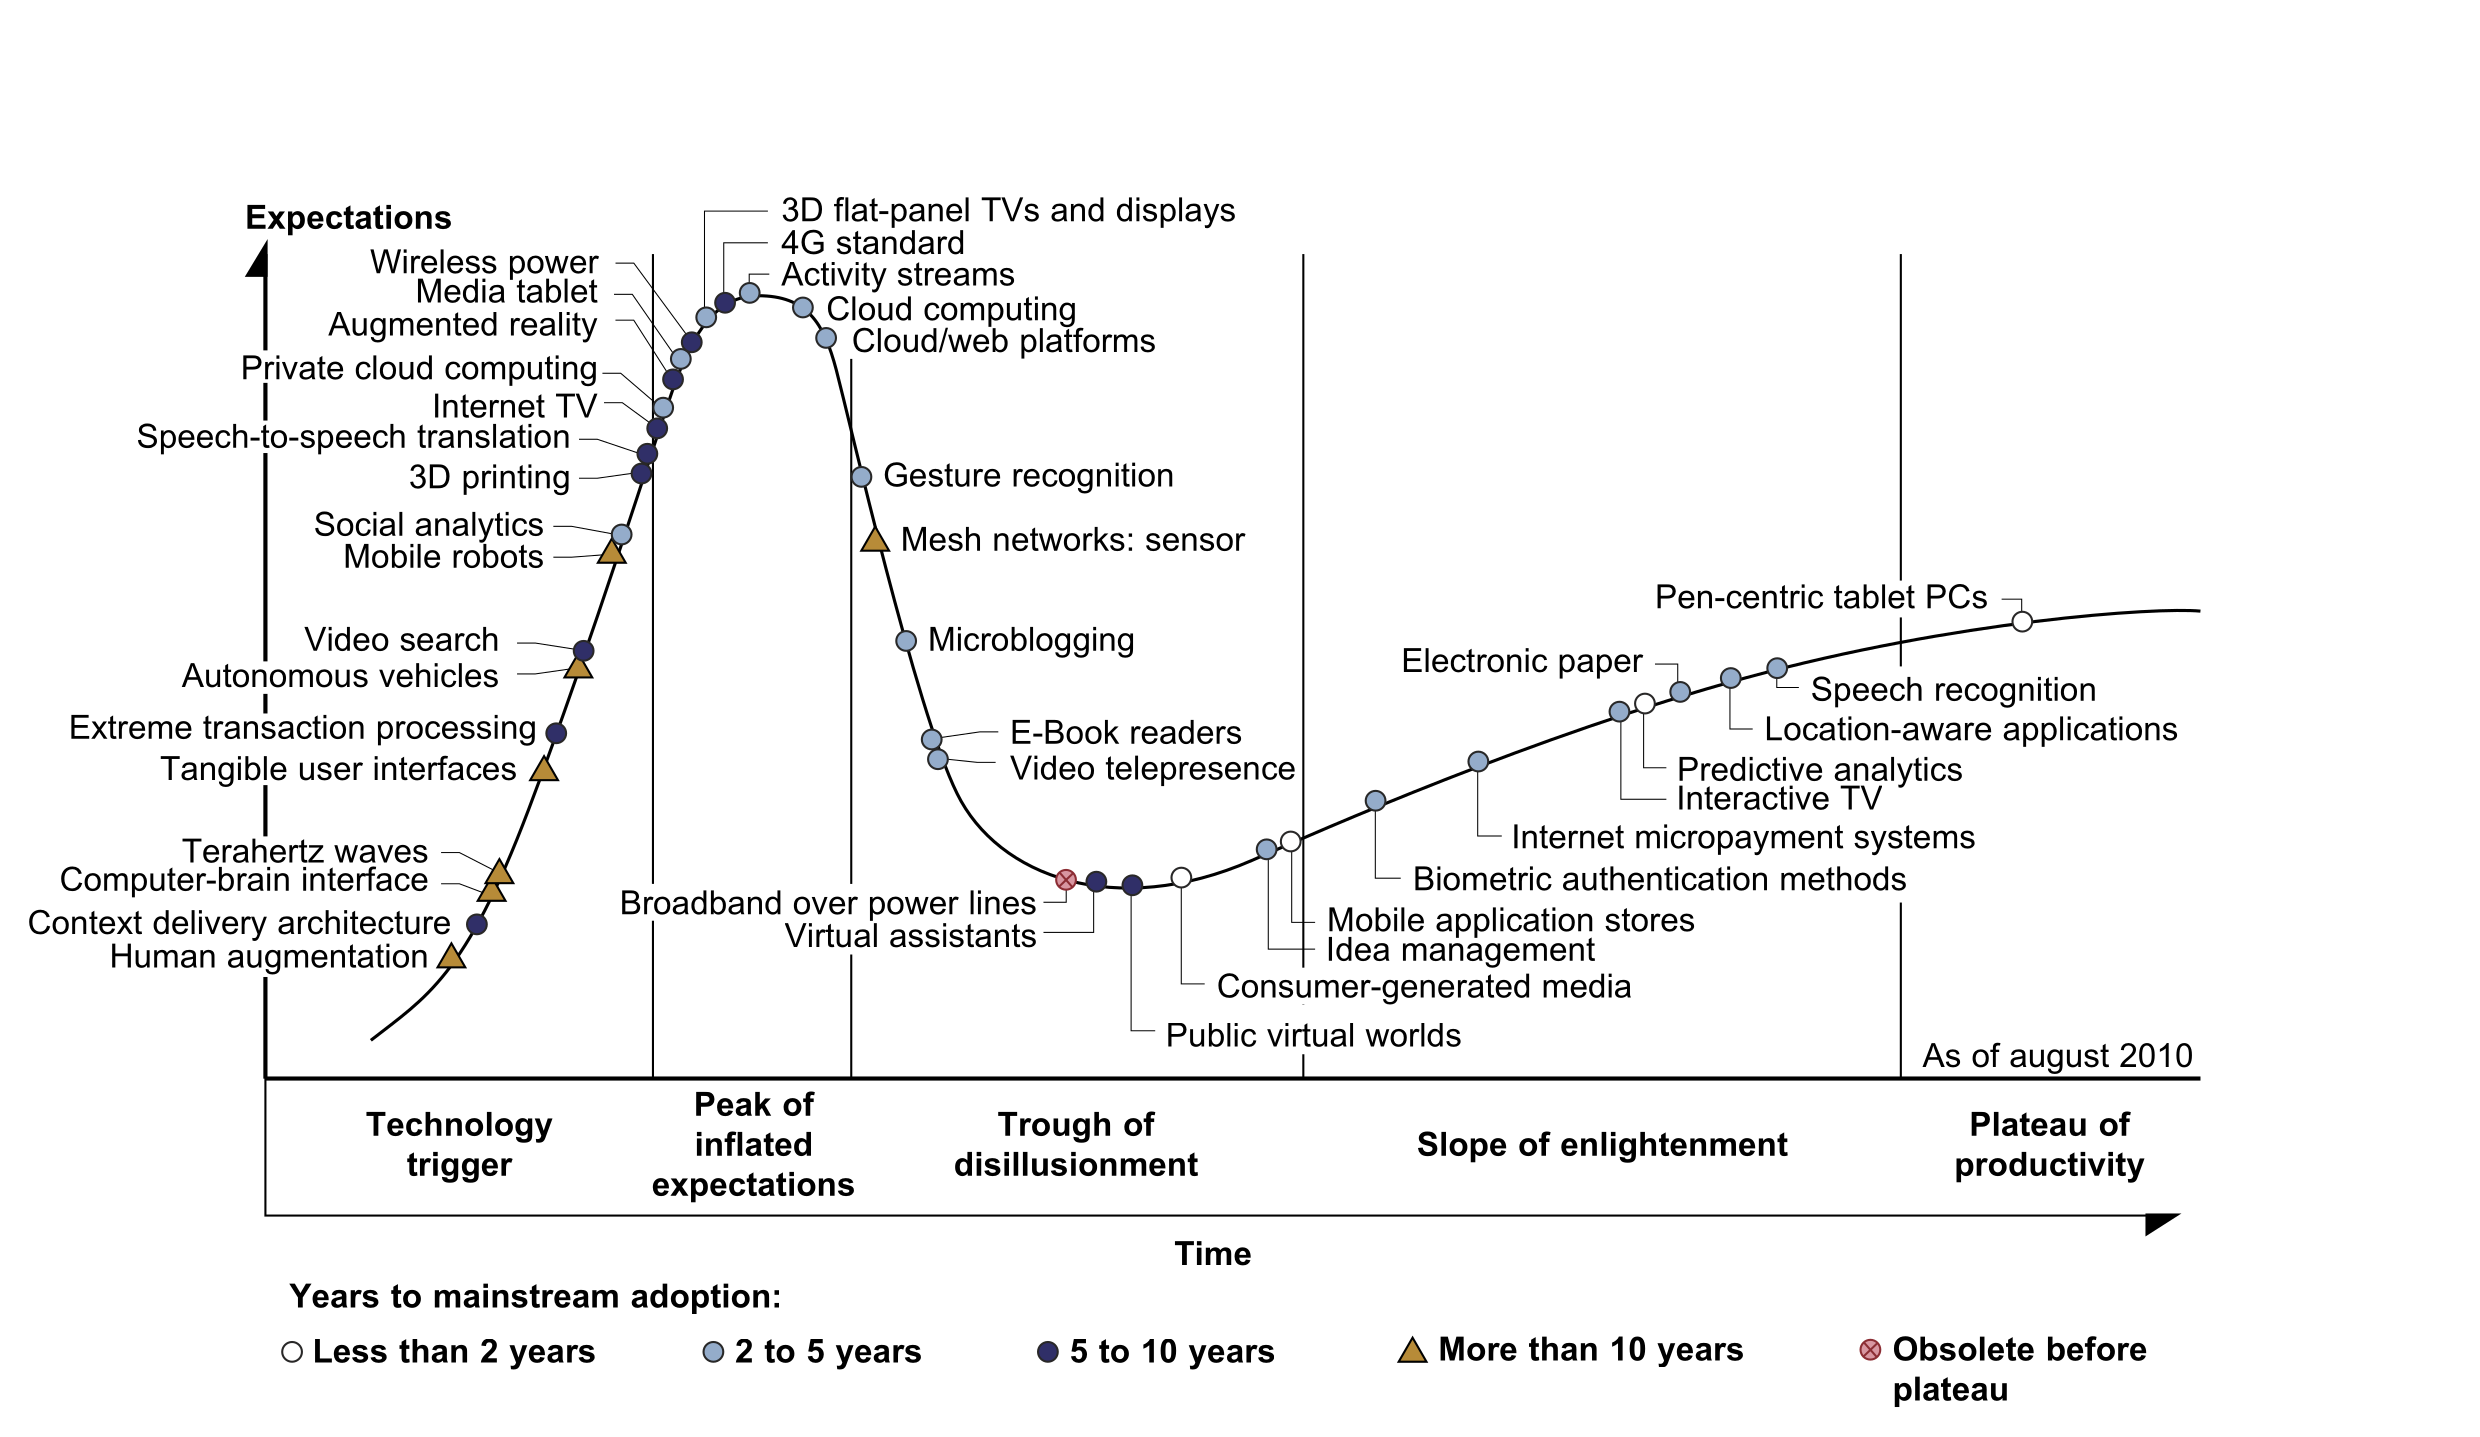
\includegraphics[width=0.85\linewidth]{images/Fig1_3_hype_cycle.png}\\
{\footnotesize Figure 1.3 of Text Book 1 (source: Gartner, Inc., 2010)}
\end{center}

\term{Hype}
{Exaggerated publicity and excitement about something.}
{}

\term{Hype Cycle}
{A graphical representation (by the research firm Gartner) of how expectations about an emerging technology change over time until it is widely adopted.}
{}

\term{Emerging Technology}
{A new technology that is still developing and not yet widely used.}
{}

\term{Mainstream Adoption}
{The stage when a technology is used widely by the general public and businesses.}
{}

%---------------------------------------------------------
\slide{46}{Five Stages of the Hype Cycle}

\begin{center}
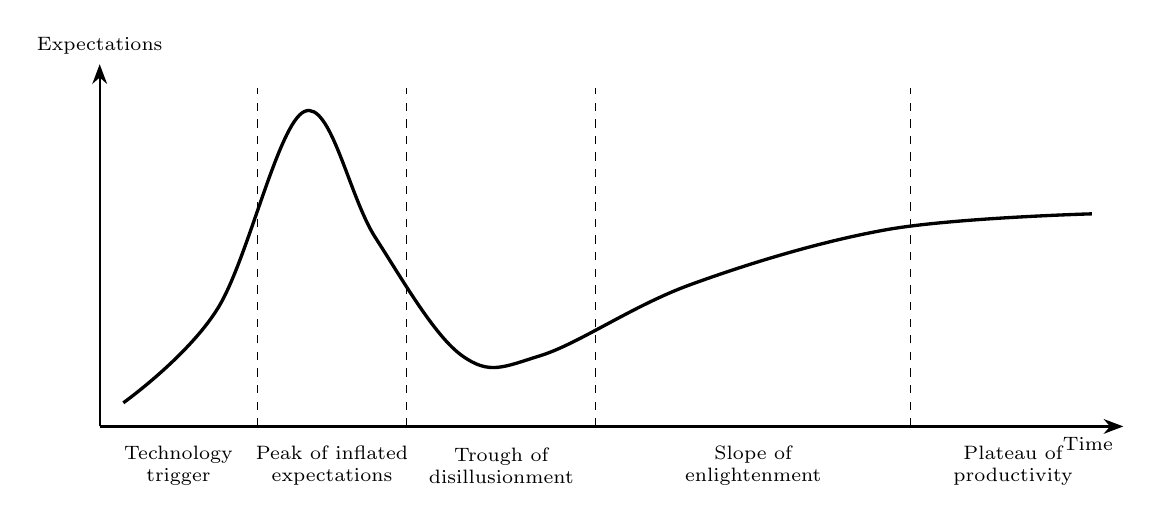
\begin{tikzpicture}[x=1cm,y=1cm]
\draw[arr] (0,0)--(13,0) node[below left,font=\scriptsize]{Time};
\draw[arr] (0,0)--(0,4.6) node[above,font=\scriptsize]{Expectations};
\draw[very thick] plot[smooth,tension=0.6] coordinates {(0.3,0.3) (1.5,1.5) (2.6,4.0) (3.5,2.4) (4.6,0.9) (5.6,0.9) (7.5,1.8) (10,2.5) (12.6,2.7)};
\foreach \x in {2,3.9,6.3,10.3} \draw[dashed] (\x,0)--(\x,4.3);
\node[font=\scriptsize,align=center] at (1,-0.5) {Technology\\trigger};
\node[font=\scriptsize,align=center] at (2.95,-0.5) {Peak of inflated\\expectations};
\node[font=\scriptsize,align=center] at (5.1,-0.5) {Trough of\\disillusionment};
\node[font=\scriptsize,align=center] at (8.3,-0.5) {Slope of\\enlightenment};
\node[font=\scriptsize,align=center] at (11.6,-0.5) {Plateau of\\productivity};
\end{tikzpicture}\\
{\footnotesize Simplified hype cycle showing its five stages.}
\end{center}

\term{Technology Trigger}
{The stage when a new technology is first introduced or demonstrated and starts attracting attention.}
{}

\term{Peak of Inflated Expectations}
{The stage when publicity is at its highest and expectations are often unrealistically high.}
{}

\term{Trough of Disillusionment}
{The stage when the technology fails to meet the inflated expectations and interest drops.}
{}

\term{Slope of Enlightenment}
{The stage when people better understand the real benefits and practical uses, and expectations rise steadily.}
{}

\term{Plateau of Productivity}
{The stage when the technology becomes stable, widely accepted, and productively used.}
{}

%---------------------------------------------------------
\slide{47}{Reading the Hype Cycle: Symbols and Examples (2010)}

\term{Years to Mainstream Adoption}
{The expected time a technology needs to reach the plateau of productivity, shown by the symbol on the curve.}
{Hollow circle: less than 2 years; gray circle: 2--5 years; dark circle: 5--10 years; triangle: more than 10 years; crossed circle: obsolete before reaching the plateau.}

\term{Obsolete}
{No longer used because it has been replaced by something better.}
{Example: broadband over power lines (2010).}

\term{Consumer-Generated Media}
{Content such as videos, reviews, and blogs created by ordinary users rather than professionals.}
{}

\term{Internet Micropayment}
{A system for making very small online payments (e.g., paying a few rupees to read an article).}
{}

\term{3D Printing}
{Making a physical object layer by layer from a digital 3D model.}
{}

\term{Mesh Network Sensors}
{Sensors that connect to each other directly in a mesh, passing data along from node to node.}
{}

\term{Broadband over Power Lines}
{Delivering high-speed Internet through ordinary electrical power cables.}
{}

\term{Biometric Authentication}
{Verifying a person's identity using physical features such as fingerprints, face, or iris.}
{Example: Aadhaar-based fingerprint authentication.}

\term{Speech Recognition}
{Technology that converts spoken words into text or commands.}
{}

\term{Predictive Analytics}
{Using data and statistical models to predict future events.}
{}

\term{Media Tablet}
{A portable touch-screen computer such as an iPad.}
{}

\term{Interactive TV}
{Television that allows viewers to interact with content (vote, shop, choose programs).}
{}

%---------------------------------------------------------
\slide{48}{Summary}

\noterms{This slide revisits terms already defined. Quick recap:}

\begin{center}
\renewcommand{\arraystretch}{1.2}
\small
\begin{tabularx}{\linewidth}{@{}lXl@{}}
\toprule
\textbf{Term} & \textbf{One-line meaning} & \textbf{Slide} \\ \midrule
HPC & Solve one big problem as fast as possible & 26 \\
HTC & Complete as many tasks as possible per unit time & 27 \\
SOA / Virtualization / IoT & Enablers of Web 2.0, clouds, and connected objects & 29 \\
Centralized computing & All resources in one system & 31 \\
Parallel computing & Many processors on one problem & 31 \\
Distributed computing & Many autonomous computers with private memory & 32 \\
Cloud computing & Resources over the Internet, centralized or distributed & 32 \\
BLP $\rightarrow$ JLP & Degrees of parallelism from bits to jobs & 38 \\
Ubiquitous, Autonomic, Composable & Common attributes of modern paradigms & 43 \\
Utility computing & Pay-per-use computing from a provider & 44 \\
Hype cycle & Five-stage curve of technology expectations & 46 \\ \bottomrule
\end{tabularx}
\end{center}

%---------------------------------------------------------
\slide{49}{Review Questions}

\noterms{No new terms. Pointers to the slides that answer each question:}

\begin{center}
\renewcommand{\arraystretch}{1.2}
\small
\begin{tabularx}{\linewidth}{@{}cXl@{}}
\toprule
\textbf{Q.} & \textbf{Question} & \textbf{Refer to} \\ \midrule
1 & Five generations of computer platforms with examples & Slide 23 \\
2 & Differentiate HPC and HTC & Slides 26--28 \\
3 & Evolutionary trend in Figure 1.1 & Slides 24--25 \\
4 & Centralized, parallel, distributed, and cloud computing & Slides 31--33 \\
5 & Three new computing paradigms and their enablers & Slide 29 \\
6 & Five degrees of parallelism & Slides 38--39 \\
7 & Vision of computer utilities (Figure 1.2) & Slides 42--44 \\
8 & Five stages of the hype cycle & Slides 45--47 \\ \bottomrule
\end{tabularx}
\end{center}

\end{document}
